%%%%%%%%%%%%%%%%%%%%%%%%%%%%%%%%%%%%%%%%%%%%%%%%%%%%%%%%%%%%%%
\chapter{FIRSTv2 au télescope Subaru}
\label{sec:FIRSTv2Subaru}
\setcounter{figure}{0}
\setcounter{table}{0}
\setcounter{equation}{0}

\minitoc

\begin{figure}[ht!]
    \centering
    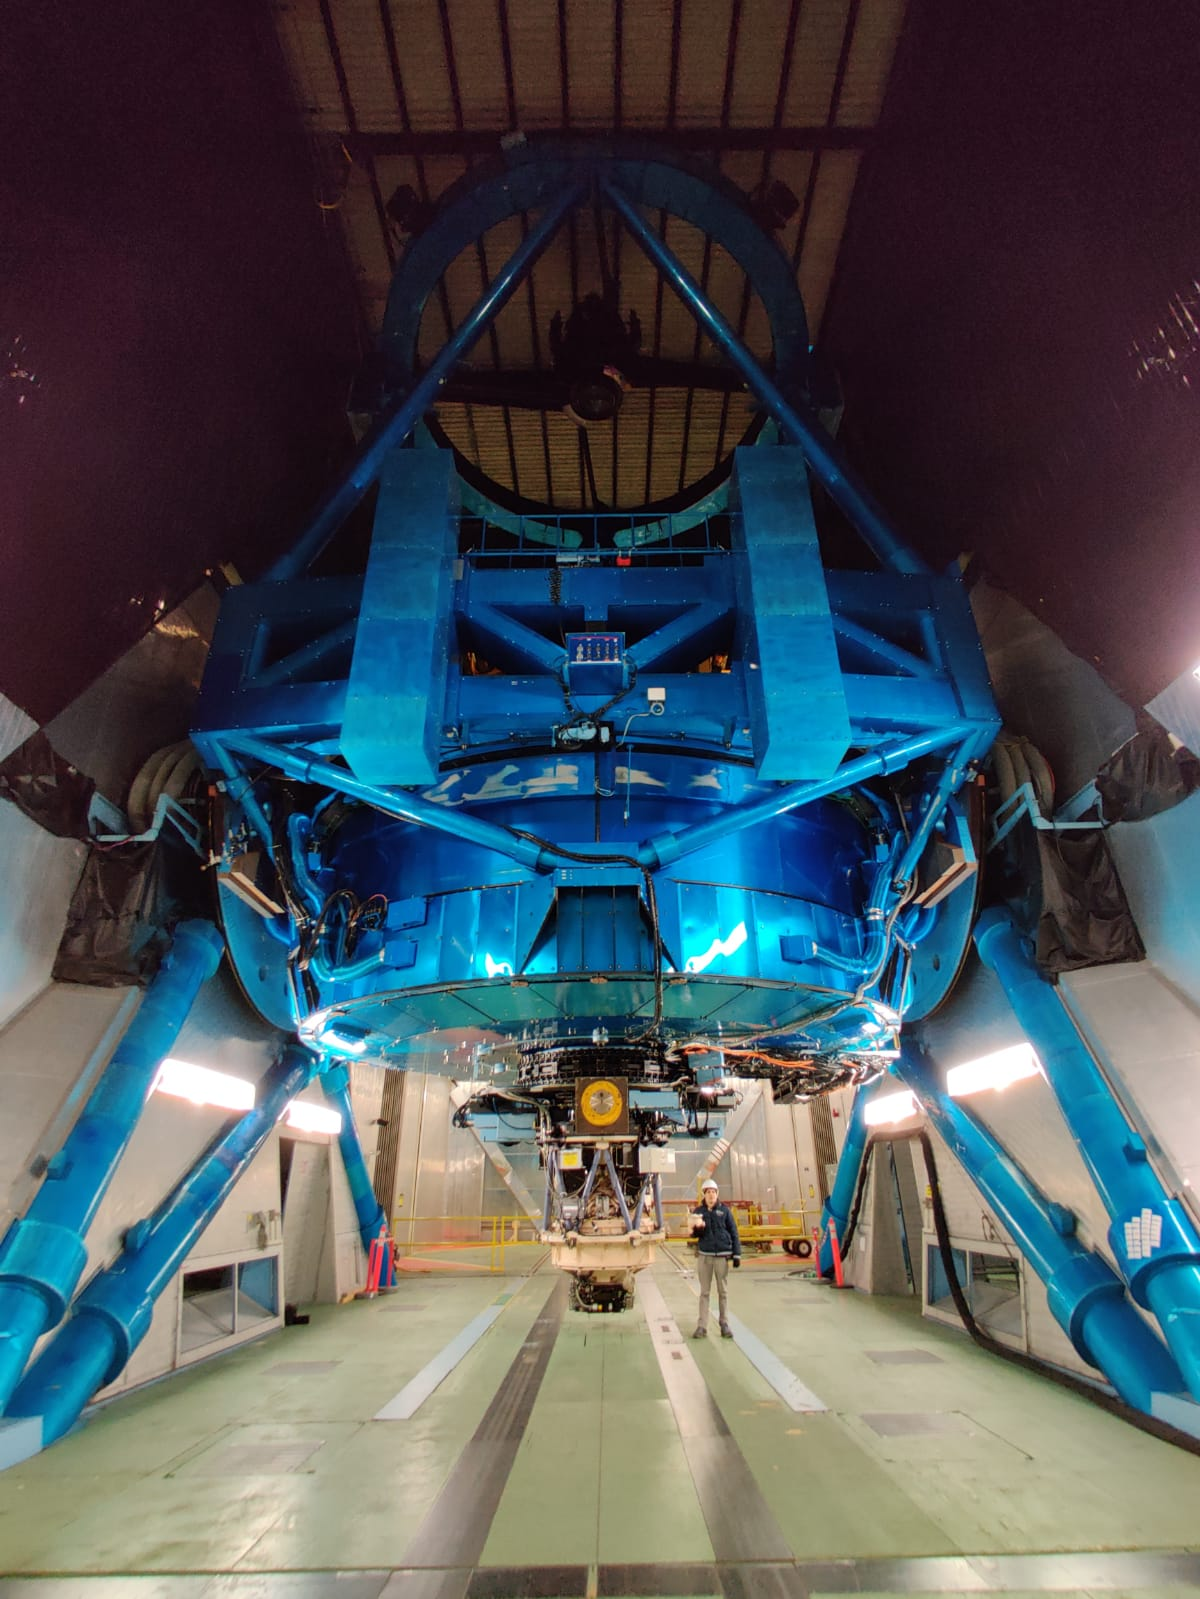
\includegraphics[width=0.47\textwidth]{Figure_Chap5/20200121_999996.jpeg}
\end{figure}

\clearpage
Durant ma thèse, j'ai participé à l'intégration de \ac{FIRSTv2} sur la plateforme \ac{SCExAO} ainsi qu'a sa première lumière le 10 septembre 2021.

Dans ce chapitre je présenterai la plateforme \ac{SCExAO} qui fournit la lumière du télescope Subaru corrigée par un système d'optique adaptative extrême (\ac{ExAO}) et permet le développement de nouveaux instruments pour l'imagerie haut contraste. à haute résolution angulaire. J'exposerai ensuite les différentes étapes d'intégration de \ac{FIRSTv2} sur la plateforme, aux côtés de \ac{FIRSTv1}. Je montre dans une troisième partie la caractérisation de \ac{FIRSTv2} sur \ac{SCExAO} et nous verrons les difficultés rencontrées. Pour finir je présenterai la première lumière et discuterai des améliorations qui ont pu être effectuées au cours des différentes nuits d'observation et tests qui ont suivi. Je conclurai enfin en présentant les développements futurs prévus sur l'instrument.


%%%%%%%%%%%%%%%%%%%%%%%%%%%%%%%%
\section{La plateforme SCExAO}

\acrfull{SCExAO} \citep{jovanovic2015} est une plateforme de R\&D pour l'imagerie \ac{HRA}, installée au foyer Nasmyth IR (voir la photographie de la figure~\ref{fig:SCExAOPhoto}) du télescope Japonais Subaru de $8,2 \,$m de diamètre. L'objectif primaire de la plateforme \ac{SCExAO} est de développer et de mettre en place un système d'optique adaptative extrême afin de fournir à plusieurs instruments un faisceau avec un haut rapport de Strehl ($80 \%$ dans la bande H) pour l'imagerie \ac{HRA}. Certains de ces instruments sont accessibles à la communauté scientifique : \acrfull{CHARIS} \citep{groff2015}, \acrfull{VAMPIRES} \citep{norris2015}, \ac{REACH} \citep{kotani2018}, \ac{MEC} \citep{walter2020} et Fast \ac{PDI} \citep{lozi2020}. D'autres sont des modules permettant le développement de nouvelles techniques pour l'imagerie \ac{HRA} : \ac{GLINT} \citep{norris2020b}, \ac{RHEA}\footnote{\url{https://www.naoj.org/Projects/SCEXAO/scexaoWEB/050devmodules.web/030rhea.web/indexm.html}} et \ac{FIRST}.

\begin{figure}[ht!]
    \centering
    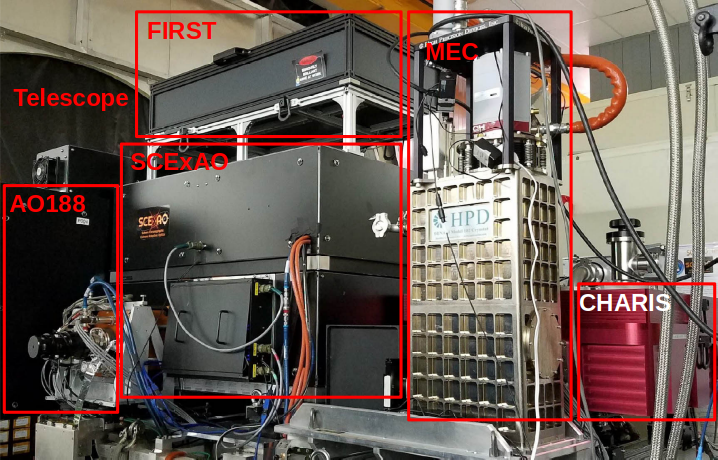
\includegraphics[width=\figwidth]{Figure_Chap5/SCExAO_onNasIR_label.png}
    \caption[Photographie de la plateforme SCExAO et des modules installés sur la plateforme Nasmyth IR du télescope Subaru.]{Photographie de la plateforme SCExAO et des modules installés sur la plateforme Nasmyth IR du télescope Subaru. Crédit : équipe SCExAO.}
    \label{fig:SCExAOPhoto}
\end{figure}

La figure~\ref{fig:SCExAOScheme} présente le schéma optique global de \ac{SCExAO}. Il est divisé en quatre blocs représentant les deux bancs infrarouge et visible de la plateforme ainsi que la source de calibration et le banc de recombinaison de \ac{FIRST}. La lumière provenant du télescope subit une première correction appliquée par l'étage d'optique adaptative AO188 \citep{minowa2010} (module en amont de \ac{SCExAO}) avec un miroir déformable comportant $188$ actionneurs.

Le faisceau corrigé est ensuite injecté sur le banc \ac{IR} (\textit{IR bench}) de \ac{SCExAO} (dans le cadre du bas de la figure~\ref{fig:SCExAOScheme}) et subit un deuxième étage de correction par un miroir déformable de $2\,000$ actionneurs (optique adaptative extrême). Puis, grâce à la dichroïque il est divisé en un faisceau visible ($< 950 \,$nm) et un faisceau \ac{IR} ($< 950 \,$nm). Ce dernier est dirigé vers les instruments travaillant dans l'\ac{IR}, indiqués par les flèches oranges sur les bords du cadre. Le faisceau lumineux passe, entre autre, par des composants (\ac{PIAA} et \textit{focal plane mask}) coronographiques (voir à ce sujet la section~\ref{sec:ImagerieDirecte}).

La partie visible du faisceau est envoyée sur le banc visible (cadre du milieu nommé \textit{visible bench}) à travers un périscope. Ce faisceau est de nouveau divisé en deux sous-faisceaux. L'un d'eux ($800 - 950 \,$nm) est analysé par le senseur de front d'onde comportant une pyramide \citep{lozi2019} et permet d'appliquer la deuxième étape de correction par optique adaptative extrême à l'aide d'un miroir déformable comportant $2\,040$ actionneurs, intégré sur le banc \ac{IR}. L'autre ($< 800 \,$nm) est injecté dans les instruments travaillant dans le visible tels que \ac{FIRST}, \ac{VAMPIRES} et \ac{RHEA}.

Le faisceau est divisé entre les instruments \ac{VAMPIRES} et \ac{RHEA} d'une part et \ac{FIRST} d'autre part. Il est dirigé dans \ac{FIRST} au niveau de la partie centrale du cadre qui contient le \ac{MEMS}, les micro-lentilles et les fibres optiques monomodes qui sont connectées au banc de recombinaison. Celui-ci est représenté dans le cadre en haut à droite, nommé \textit{FIRST recombination} et il contient les deux versions de \ac{FIRST}. Il s'agit de sa configuration actuelle, qui est légèrement différente mais équivalente à celle présentée sur le schéma du bas de la figure~\ref{fig:FIRSTV1V2FinalScheme} de la section~\ref{sec:V1V2Subaru}.

Enfin, le cadre de gauche en haut de la figure~\ref{fig:SCExAOScheme} présente le banc des différentes sources internes, notamment la source super continuum ($600 - 2500 \,$nm) qui est utilisée pour simuler un point source vu par \ac{SCExAO} servant pour les tests et l'étalonnage de la \ac{P2VM}. Ces sources sont injectées via une fibre optique sur la plateforme \ac{SCExAO} par le banc \ac{IR} (cadre du bas), au niveau de l'injection du faisceau du télescope. De cette façon, la source lumineuse parcourt toute la plateforme jusqu'aux instruments.

\begin{figure}[ht!]
    \centering
    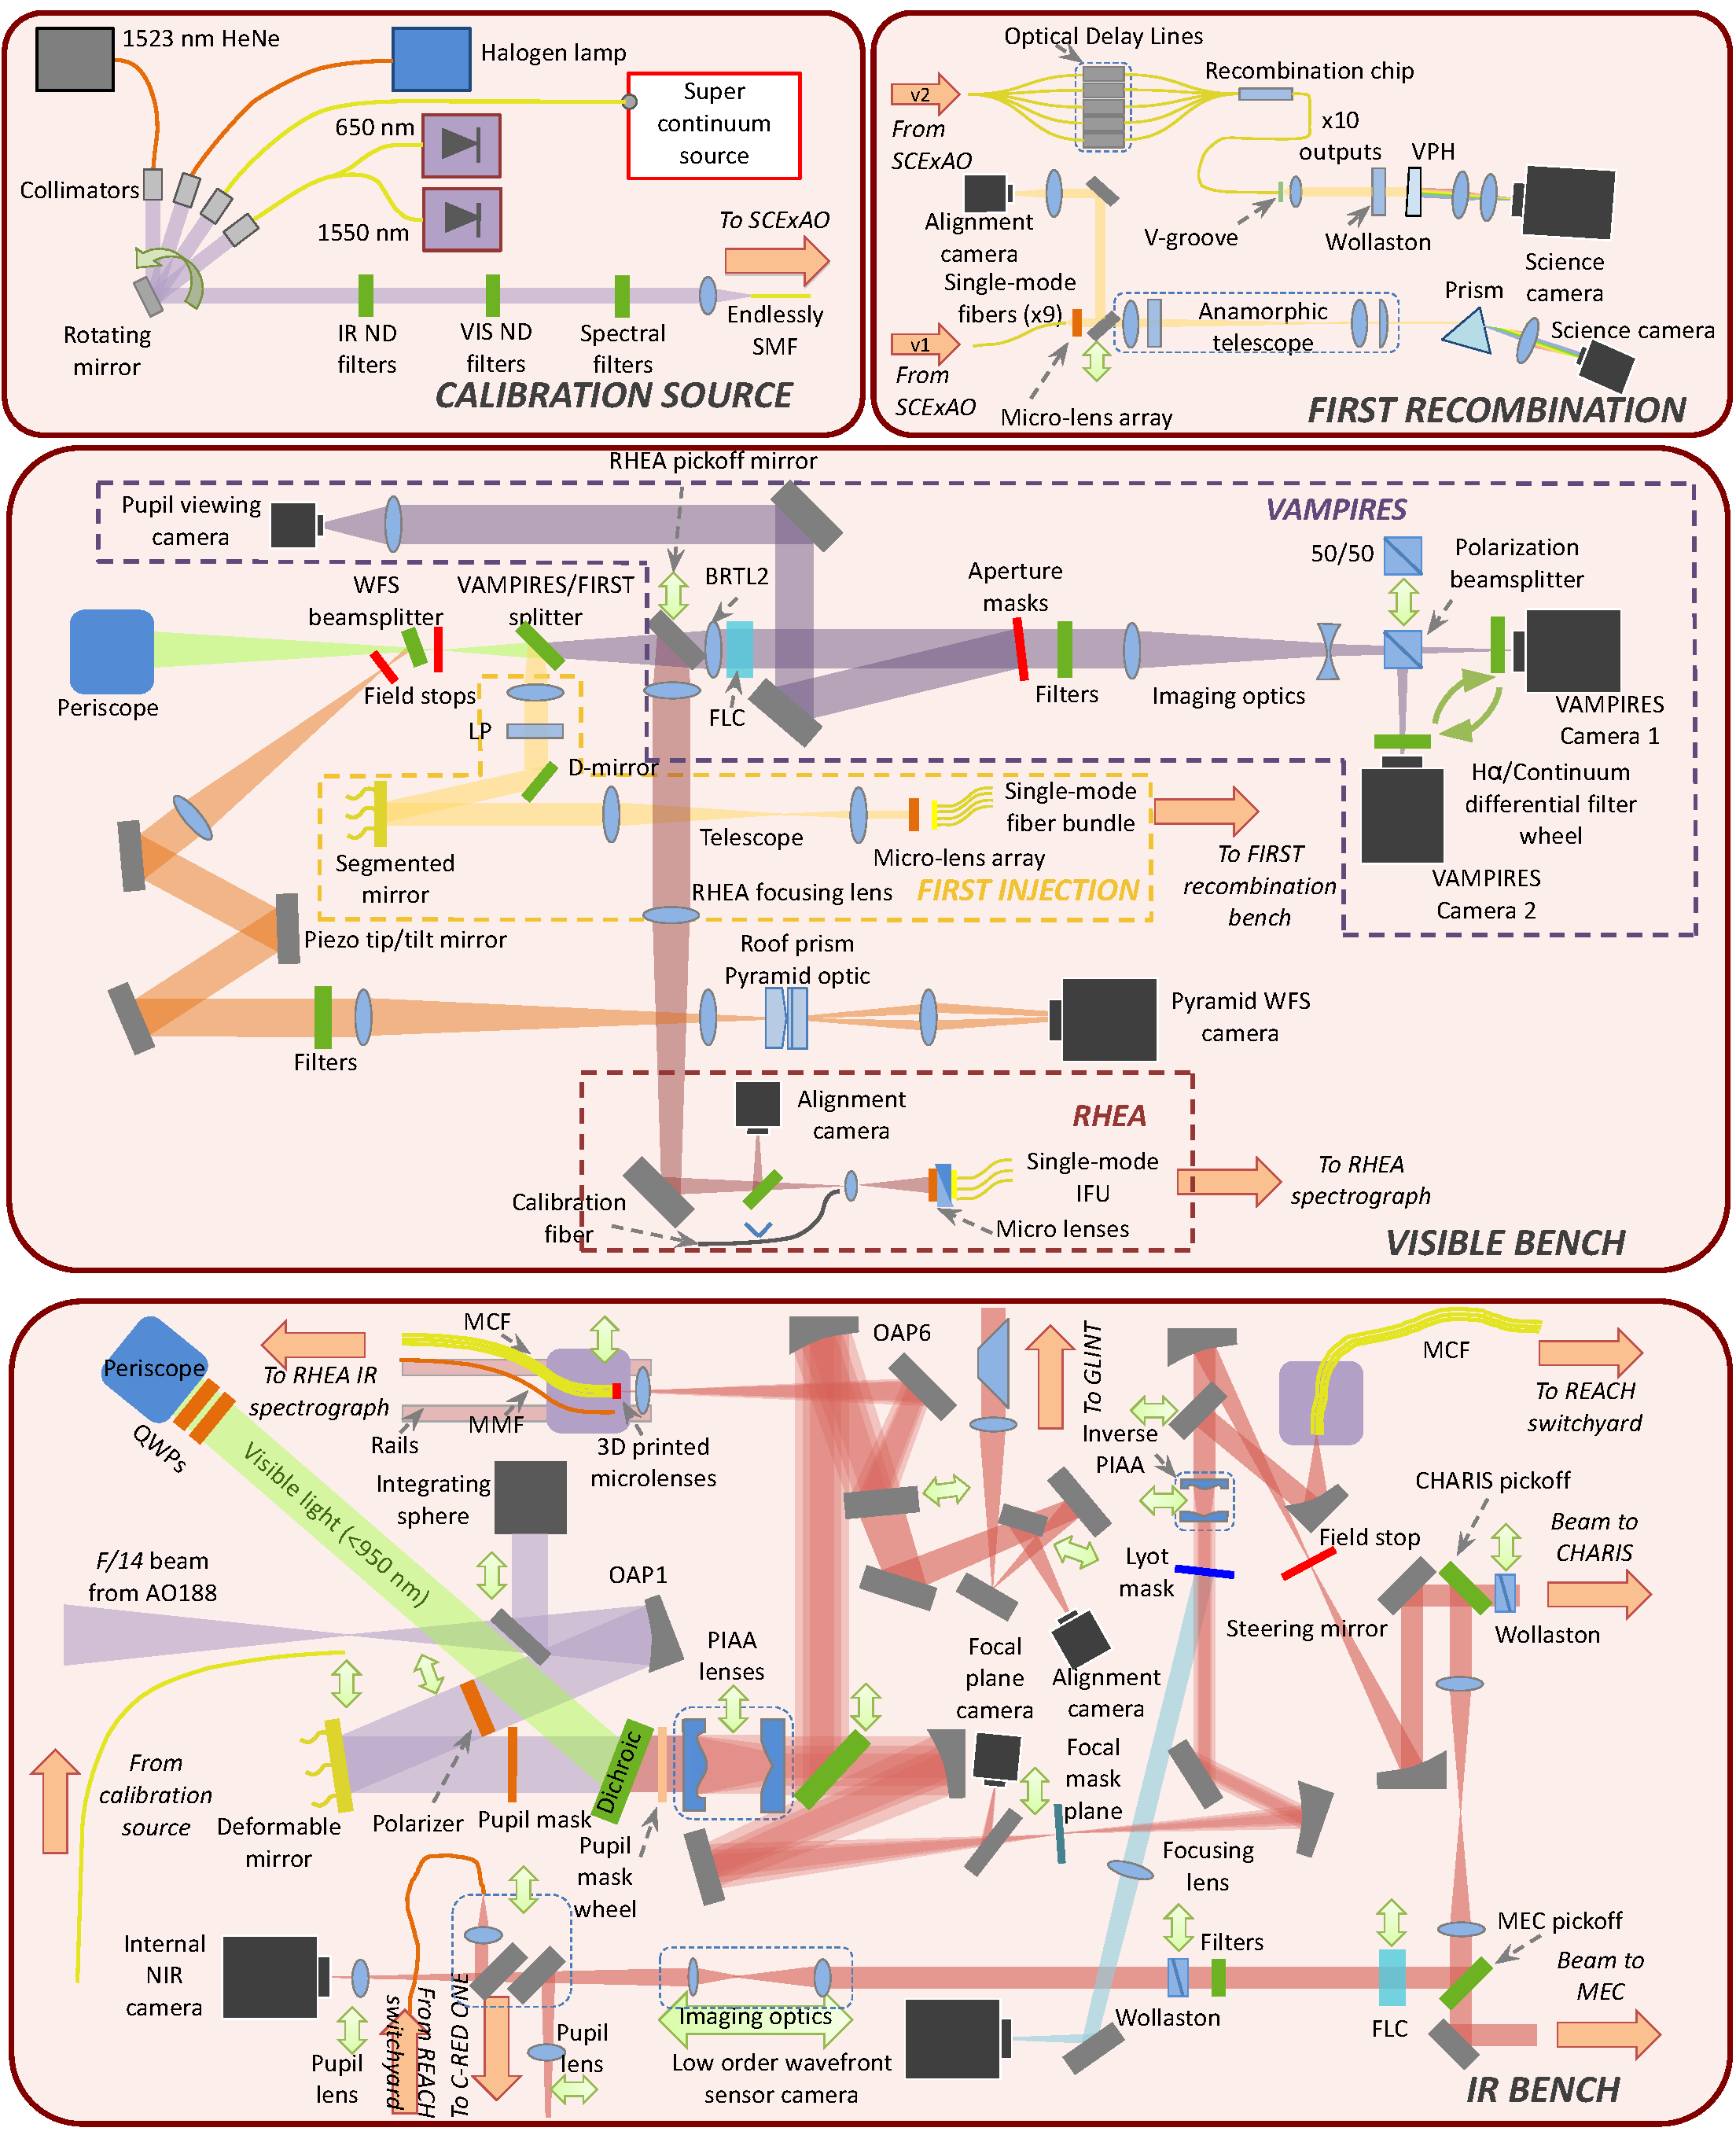
\includegraphics[width=0.89\textwidth]{Figure_Chap5/20230212_FullBench.pdf}
    \caption[Schéma de principe de la plateforme SCExAO.]{Schéma de principe de la plateforme SCExAO. L'entrée se situe sur le banc infrarouge nommé \textit{IR bench} (cadre du bas). Le faisceau est divisé en une voie visible ($< 950 \,$nm) et en une voie infrarouge (IR) dirigée vers les instruments travaillant dans l'IR (GLINT, REACH, CHARIS, MEC, RHEA). La voie visible est envoyée sur le banc visible nommé \textit{visible bench} (cadre du milieu) via un périscope, est divisée et dirigée vers le senseur de front d'onde pour l'ExAO et vers les instruments travaillant dans le visible (FIRST, VAMPIRES, RHEA). Le faisceau est injecté dans FIRST (au centre) et les deux versions de recombinaison (v1 et v2) sont sur le banc nommé \textit{FIRST recombination} (cadre en haut à droite). Le banc des sources de calibration nommé \textit{calibration source} (cadre en haut à gauche) permet d'injecter différentes sources à l'entrée de SCExAO. Crédit : équipe SCExAO.}
    \label{fig:SCExAOScheme}
\end{figure}

On peut voir les différents bancs mentionnés (excepté celui de la source de calibration) sur la photo de la figure~\ref{fig:SCExAOPhoto}. En effet, ils sont montés les uns sur les autres, du banc \ac{IR} jusqu'au banc de recombinaison de \ac{FIRST}, de bas en haut.


%%%%%%%%%%%%%%%%%%%%%%%%%%%%%%%%
\section{Intégration de FIRSTv2 sur SCExAO}

Deux missions à Hawaï m'ont permis d'intégrer une partie de \ac{FIRSTv2} sur le télescope Subaru. Durant la première mission, se déroulant deux semaines en janvier 2020, j'ai déployé le nouveau logiciel de contrôle que j'avais développé en laboratoire, tout en intégrant la caméra \ac{EMCCD} Andor Ixon (voir plus loin). J'ai ainsi participé à une nuit d'observation (ma toute première) le 30 janvier 2020 permettant de tester la nouvelle installation de \ac{FIRSTv1} sur l'étoile $\upbeta$ Ori. Pendant la deuxième mission, se déroulant tout le mois de février 2022, j'ai intégré la puce $Y$ que j'ai testée au préalable sur le banc de test à Meudon. Trois nuits d'observation ont permis d'acquérir des données avec cette puce.

Le bon déroulement des intégrations et des nuits d'observation a pu être possible grâce à \textbf{l'aide et au travail précieux} de Sébastien Vievard avec qui j'ai beaucoup collaboré à distance (en partie à cause des limitations de la pandémie de COVID-19 sur les missions). Il a ainsi intégré les \acrshort{ODL}s et la puce $X$ (envoyée par colis depuis Meudon) s'assurant que la première lumière de \ac{FIRSTv2} ait bien lieu en septembre 2021.


%%%%%%%%%%%%%%%%
\subsection{Premières étapes d'installation}
\label{sec:V1V2Integration}

% Intégration de la caméra Ixion pendant ma première mission en 2020
Lors de ma première mission à Hawaï, en janvier 2020, j'ai déployé le logiciel de contrôle que j'avais commencé à développer sur le banc de test à Meudon (voir plus de détails sur le logiciel dans la section~\ref{sec:ControlSoftware}). Dans le même temps, Sébastien Vievard a intégré sur l'instrument \ac{FIRSTv1} la caméra de la gamme Andor Ixon Ultra $897$ fabriquée par \textit{Oxford Instruments}. Elle dispose d'un capteur de la technologie \acrfull{EMCCD} de $512 \,\text{px} \times 512\,\text{px}$ de taille égale à $16 \,$\um. On a fait face à des difficultés pour l'acquisition des images et, avec l'aide de Barnaby Norris, on a pu trouver une procédure qui menait à bien l'acquisition de cubes d'images. De plus, la caméra Ixon était en conflit avec la caméra photométrique du même fabricant, de la gamme Andor Luca, lorsque les deux étaient simultanément connectées à l'ordinateur. La solution a été d'alimenter les caméras par des prises dont l'alimentation est contrôlable à distance. On a fini par tester et valider la nouvelle installation de \ac{FIRSTv1} en observant l'étoile $\upbeta$ Ori lors de la nuit du 30 janvier 2020.

% Intégration des ODLs pendant l'été 2021
L'intégration de \ac{FIRSTv2} a continué par l'achat et l'intégration des lignes à retard (\acrfull{ODL}). Sébastien Vievard s'est chargé de commander auprès de \textit{Oz Optics} cinq \ac{ODL}s du même modèle que celles dont nous disposons à Meudon (voir plus de détails dans la section~\ref{sec:InstruODL}) avant de fabriquer l'interface électronique et de les intégrer sur \ac{FIRSTv1} pendant l'été 2021. La différence de sensibilité de l'instrument lors de tests sur la source interne nous a paru conséquente et il a été décidé de mesurer leur transmission, estimée à $20 - 30 \%$. Cette faible transmission est bien inférieure à celle spécifiée ($\sim 75 \%$ à $650 \,$nm) et nous avons donc décidé de conduire les mêmes mesures à Meudon (pour cela voir la section~\ref{sec:OdlThroughput}). C'est un point très préoccupant car cela va à l'encontre de notre objectif de gagner en sensibilité avec \ac{FIRSTv2}. On a ainsi commencé à envisager de redéfinir le concept de l'instrument pour se débarrasser, à terme, des \ac{ODL}s, comme j'ai pu en discuter dans la section~\ref{sec:ODLDiscussions}.

% Intégration de la puce X pendant l'été 2021
% Les nuits d'observations entre 20210910 et <20220214 sont sur Ixion, v2 seul
Dans le même temps, la puce $X$ a été envoyée à Hawaï depuis Meudon pour finir l'intégration des éléments de \ac{FIRSTv2} et la première lumière a pu avoir lieu le 10 septembre 2021. La figure~\ref{fig:FIRSTV1V2IxonPhoto} présente une photographie du banc de recombinaison de \ac{FIRST} en février 2022, après la ré-intégration en parallèle de \ac{FIRSTv1}. Dans le coin en haut à gauche se trouve la puce photonique protégée par une feuille de papier optique, sur une petite plateforme montée au dessus des \ac{ODL}s (non visibles) connectées à l'ordinateur de contrôle par les câbles blancs sur la partie haute. La puce est connectée aux fibres du V-Groove installé sur la partie centre gauche de la photographie, devant l'objectif de microscope. Le faisceau en sortie de ce dernier est tracé en bleu et traverse d'abord le prisme de Wollaston avant d'être dispersé par un prisme. Une lentille image le faisceau sur la caméra en haut à droite. Le faisceau de \ac{FIRSTv1} est tracé en rouge au niveau de l'entrée du système anamorphique et est dispersé par un autre prisme, en bas de la photographie. Le faisceau est ensuite réfléchi par deux miroirs plans et imagé par une lentille sur la même caméra que précédemment. Les images acquises contiennent alors les interférogrammes des deux versions de l'instrument (voir la figure~\ref{fig:V1V2Image}), ce qui a permis une estimation de leur différence de sensibilité, présentée plus loin dans la section~\ref{sec:V1V2Throughput}.

% Entre 20220214 et <=20220302, imagerie simultanée de v1 et v2 sur Ixion
\begin{figure}[ht!]
    \centering
    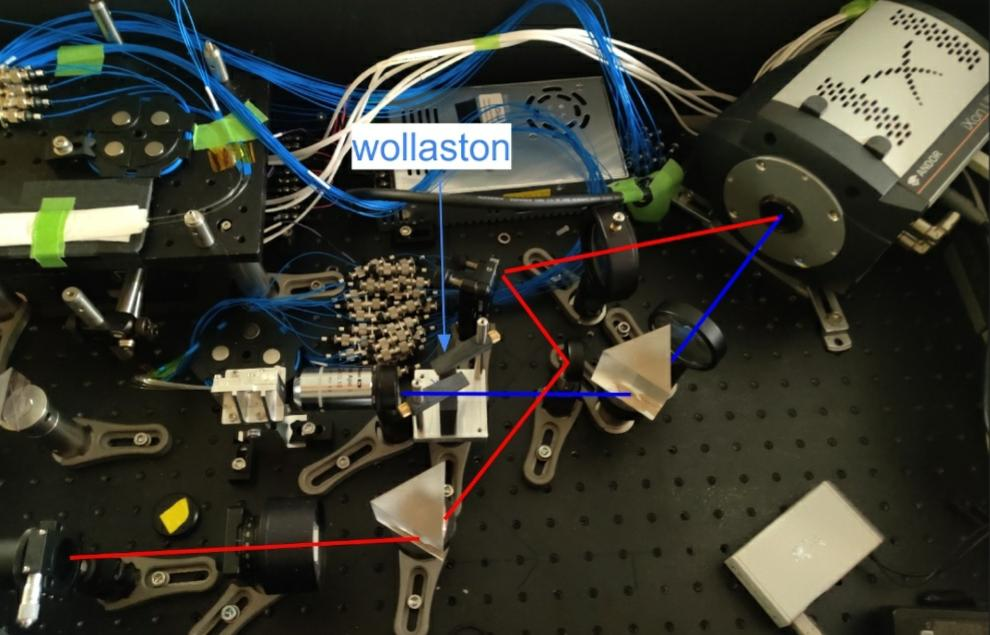
\includegraphics[width=\figwidth]{Figure_Chap5/20220201_Subaru_V1V2.jpeg}
    \caption[Photographie des deux versions de FIRST installées sur le banc de recombinaison de SCExAO, partageant la même caméra.]{Photographie des deux versions de FIRST installées sur le banc de recombinaison de SCExAO, partageant la même caméra. La puce $X$ (en haut à gauche) est enroulée dans du papier optique sur une plateforme au-dessus des ODLs et ses fibres de sortie sont connectées aux fibres du V-Groove (centre gauche). Le faisceau de FIRSTv2 est tracé en bleu en sortie de l'objectif de microscope placé devant les sorties du V-Groove, traverse le prisme de Wollaston et est dispersé par un prisme. Une lentille image ensuite le faisceau sur la caméra Andor Ixon (en haut à droite). Le faisceau de FIRSTv1 est tracé en rouge en bas à gauche, en entrée du système anamorphique et est dispersé par un prisme avant d'être réfléchi par deux miroirs plans et imagé par une lentille sur la même caméra. Crédit : Sébastien Vievard.}
    \label{fig:FIRSTV1V2IxonPhoto}
\end{figure}

\begin{figure}[ht!]
    \centering
    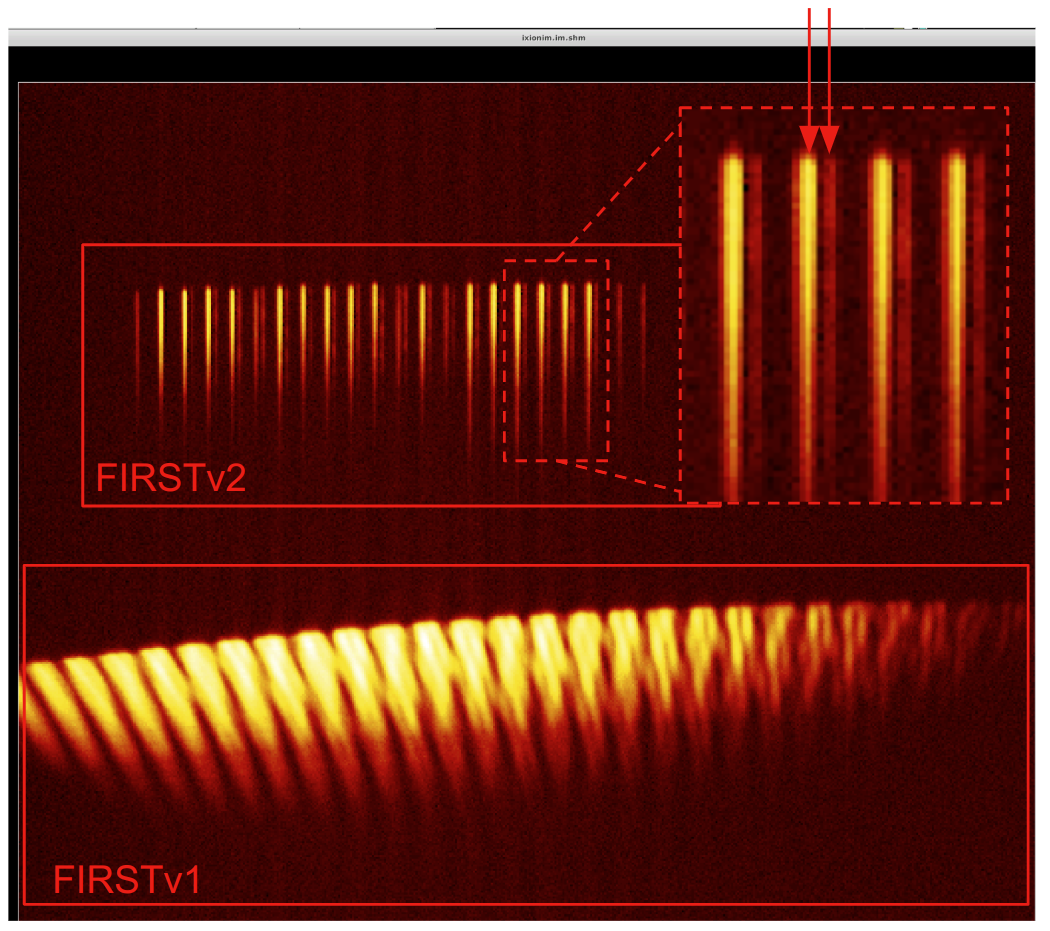
\includegraphics[width=\figwidth]{Figure_Chap5/image_2023_02_21T23_27_17_685Z.png}
    \caption[Images des interférogrammes de FIRSTv1 et FIRSTv2 sur la caméra Andor Ixon sur source interne.]{Images des interférogrammes de FIRSTv1 (en bas) et FIRSTv2 (en haut) sur la caméra Andor Ixon sur source interne. Les OPDs ne sont pas annulées sur les voies de FIRSTv2 et aucune frange n'apparaît sur les sorties correspondantes. Un agrandissement de quatre des sorties de V2 est montré pour mettre en évidence les sorties sélectionnées par le prisme de Wollaston dans la polarisation verticale (flèche rouge de gauche) et horizontale (flèche rouge de droite). Crédit : Sébastien Vievard.}
    \label{fig:V1V2Image}
\end{figure}

% Intégration de la puce Y pendant ma deuxième mission en février 2022
Ma deuxième mission, en février 2022, a été l'occasion d'intégrer la puce $Y$ sur le banc de recombinaison et de la tester lors de plusieurs nuits d'observations. De plus, j'ai également intégré un prisme de Wollaston ce qui nous a permis d'améliorer la qualité des données en traitant les deux polarisations séparément. Enfin, j'ai été amené à améliorer la procédure de prise de données au niveau de la synchronisation de la caméra et du \ac{MEMS}, le logiciel à Hawaï étant différent de celui à Meudon. Mais aussi, je me suis rendu compte que la procédure de prise de données n'assurait pas la connaissance de l'étape de modulation pour chaque image, ce qui est primordial pour le traitement de données. Pour ce faire, il a fallu assigner un entier à chaque étape de la séquence de modulation qui était enregistré dans un pixel d'un des coins des images. En effet, contrairement à la procédure d'acquisition à Hawaï, celle au laboratoire à Meudon est telle que la première image de chaque séquence acquise correspond nécessairement à la première étape de la séquence de modulation, ce qui dispensait de se préoccuper de ce sujet.


%%%%%%%%%%%%%%%%
\subsection{Augmentation de la résolution spectrale}
\label{sec:V1V2Subaru}

% Intégration du nouveau spectro et de la nouvelle caméra de V2 (>20220309) + ré-intégration de V1 (>=20220427)
En mars 2022, Sébastien Vievard et Manon Lallement ont procédé au réalignement des deux versions de \ac{FIRST}, à la suite de la réception d'une nouvelle caméra (présentée ci-après) et des optiques du nouveau concept de spectro-imageur, conçu par Manon Lallement (voir plus de détails dans la section~\ref{sec:InstruSpectro}). La nouvelle configuration est illustrée par le schéma de principe de la figure~\ref{fig:FIRSTV1V2FinalScheme} qui représente le banc de recombinaison de \ac{FIRST}. De manière similaire à la photographie de la figure~\ref{fig:FIRSTV1V2IxonPhoto} présentée précédemment, les fibres proviennent du banc visible par la gauche et neuf d'entre elles sont connectées sur les fibres du V-Groove de \ac{FIRSTv1} (en bas à gauche), disposé devant une matrice de micro-lentilles qui collimatent les faisceaux de sortie. Ces derniers peuvent être dirigés par un miroir plan contrôlable en position vers le système d'imagerie photométrique pour l'optimisation de l'injection du flux dans les fibres par le \ac{MEMS} (sur le banc visible), ou vers la partie recombinaison interférométrique composée du système anamorphique, de deux miroirs plans, du prisme, de la lentille d'imagerie et de la caméra de science (Andor Ixon, en haut à droite). En parallèle, cinq des fibres provenant du banc visible sont connectées aux \ac{ODL}s de \ac{FIRSTv2} (en haut à gauche) dont les fibres de sortie sont connectées à celles en entrée de la puce photonique (en haut au centre). Les fibres de sortie de cette dernière sont connectées aux fibres du V-Groove (au centre) et les faisceaux sont collimatés par l'objectif de microscope, traversent le prisme de Wollaston, sont dispersés par le nouveau spectro-imageur (composé d'un réseau holographique et de deux lentilles) et sont imagés sur la nouvelle caméra.

% Schéma final du banc de recombinaison
\begin{figure}[ht!]
    \centering
    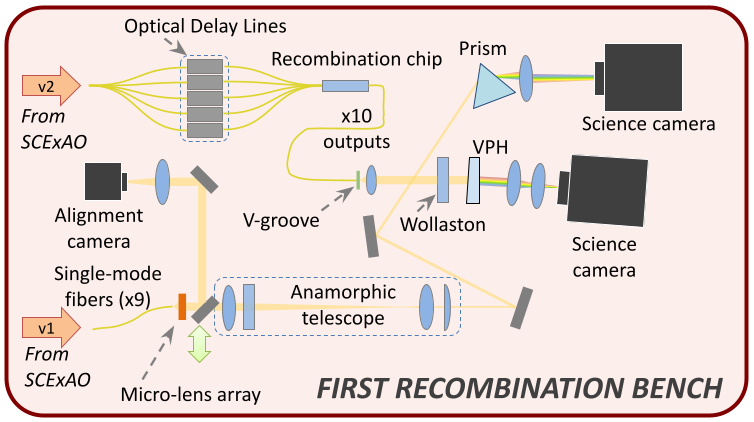
\includegraphics[width=\figwidth]{Figure_Chap5/20220601_SCExAO_FIRSTRecombBench_V1_V2_Scheme.png}
    \caption[Schéma de principe des deux versions de FIRST installées en parallèle sur le banc de recombinaison de SCExAO.]{Schéma de principe des deux versions de FIRST installées en parallèle sur le banc de recombinaison de SCExAO. Les $9$ fibres de v1 provenant du banc visible (en bas à gauche) sont connectées aux fibres d'un V-Groove dont les faisceaux de sortie sont collimatés par une matrice de micro-lentilles, puis peuvent être orientés par un miroir plan mobile vers la voie photométrique ou vers la voie interférométrique. Celle-ci est composée (du coin en bas à gauche vers le coin en haut à droite) d'un système anamorphique, de 2 miroirs plans, d'un prisme dispersant, d'une lentille d'imagerie et de la caméra (Andor Ixon). Les 5 fibres de v2 provenant du banc visible (en haut à gauche) sont connectées aux ODLs, elles-mêmes connectées à la puce photonique, elle-même connectée au V-Groove (au centre). Puis se trouvent un objectif de microscope, un prisme de Wollaston, un réseau holographique, deux lentilles d'imagerie et la caméra (Hamamatsu). Crédit : Sébastien Vievard.}
    \label{fig:FIRSTV1V2FinalScheme}
\end{figure}

% Intégration de la nouvelle caméra Orca à partir du 9 mars 2022 (données >=20220323) en parallele de V1
% Hamamatsu Orca Quest qCMOS camera: https://www.hamamatsu.com/eu/en/product/type/C15550-20UP/index.html
La nouvelle caméra d'imagerie scientifique de \ac{FIRSTv2} est de la gamme Orca Quest qCMOS fabriquée par \textit{Hamamatsu}\footnote{\url{https://www.hamamatsu.com/}}. De même que la caméra à Meudon, elle dispose d'un capteur de la technologie \ac{CMOS}, de $4\,000 \,\text{px} \times 2\,300 \,$px de taille égale à $4,6 \,$\um. Sa bande passante est $300 - 1000 \,$nm avec une efficacité quantique de $80 - 65\%$ sur la gamme spectrale $600 - 700 \,$nm. Le bruit sur le courant d'obscurité lorsqu'elle est refroidie à l'eau (température du capteur de $-35\degree \,$C) vaut $0,006 \,\text{e}^-.px^{-1}.s^{-1}$ et le bruit de lecture est de $0,25 - 0,4 \,\text{e}^-$ suivant le mode de lecture, ce qui est mieux d'un facteur $\sim 24$ et d'un facteur $\sim 3$, respectivement, par rapport à celle de la gamme Andor Zyla à Meudon. La taille plus petite des pixels de cette caméra (d'un facteur $\sim 3,5$) permet d'obtenir la résolution spectrale estimée dans le prochain paragraphe.

% Intégration du nouveau spectro à partir du 9 mars 2022 (données >=20220323)
Dans le même temps, le spectro-imageur conçu à Meudon par Manon Lallement (pour plus de détails voir la section~\ref{sec:InstruSpectro}) est intégré à \ac{FIRSTv2} et est indiqué par la mention \acrshort{VPH} (\acrlong{VPH}) sur le schéma de la figure~\ref{fig:FIRSTV1V2FinalScheme}. Un étalonnage spectral à partir de la source d'étalonnage de l'instrument \ac{CHARIS} (dont la longueur d'onde est ajustable grâce à un filtre ajustable) permet d'estimer la résolution spectrale du spectro-imageur à $\sim 3\,000$ à $650 \,$nm. L'identification en longueur d'onde des raies dans le flux mesuré et son ajustement polynomial sont présentés sur le graphique du haut et du bas de la figure~\ref{fig:V2SpecCalSubaru}, respectivement. De même que l'étalonnage spectral effectué à Meudon et présenté dans la section~\ref{sec:EtalonnageSpectral}, la fonction polynomiale de l'ajustement de la longueur d'onde sur les pixels de la caméra est linéaire et la résolution spectrale est similaire.

\begin{figure}[ht!]
    \centering
    \begin{subfigure}{\textwidth}
        \centering
        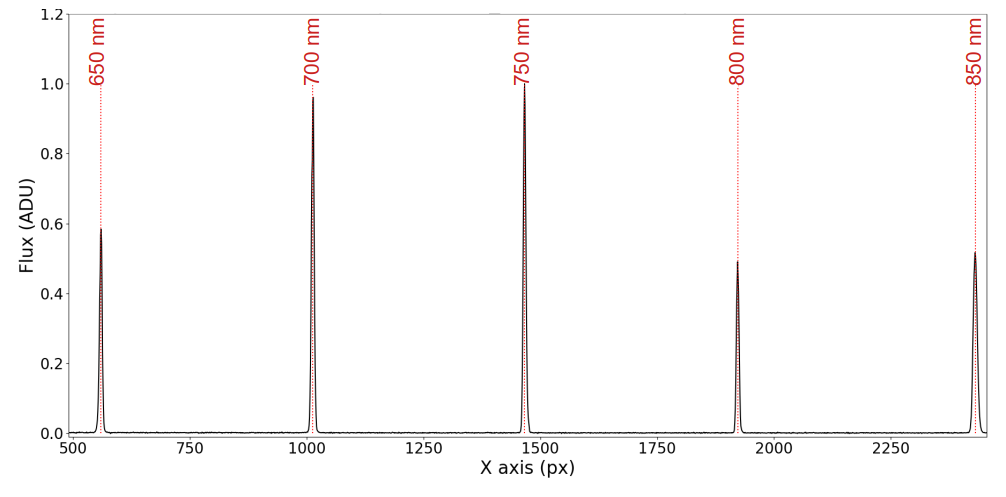
\includegraphics[width=\textwidth]{Figure_Chap5/20220404_5TC_PY_SpectralCalFlux01_Crop.png}
    \end{subfigure}
    \begin{subfigure}{\textwidth}
        \centering
        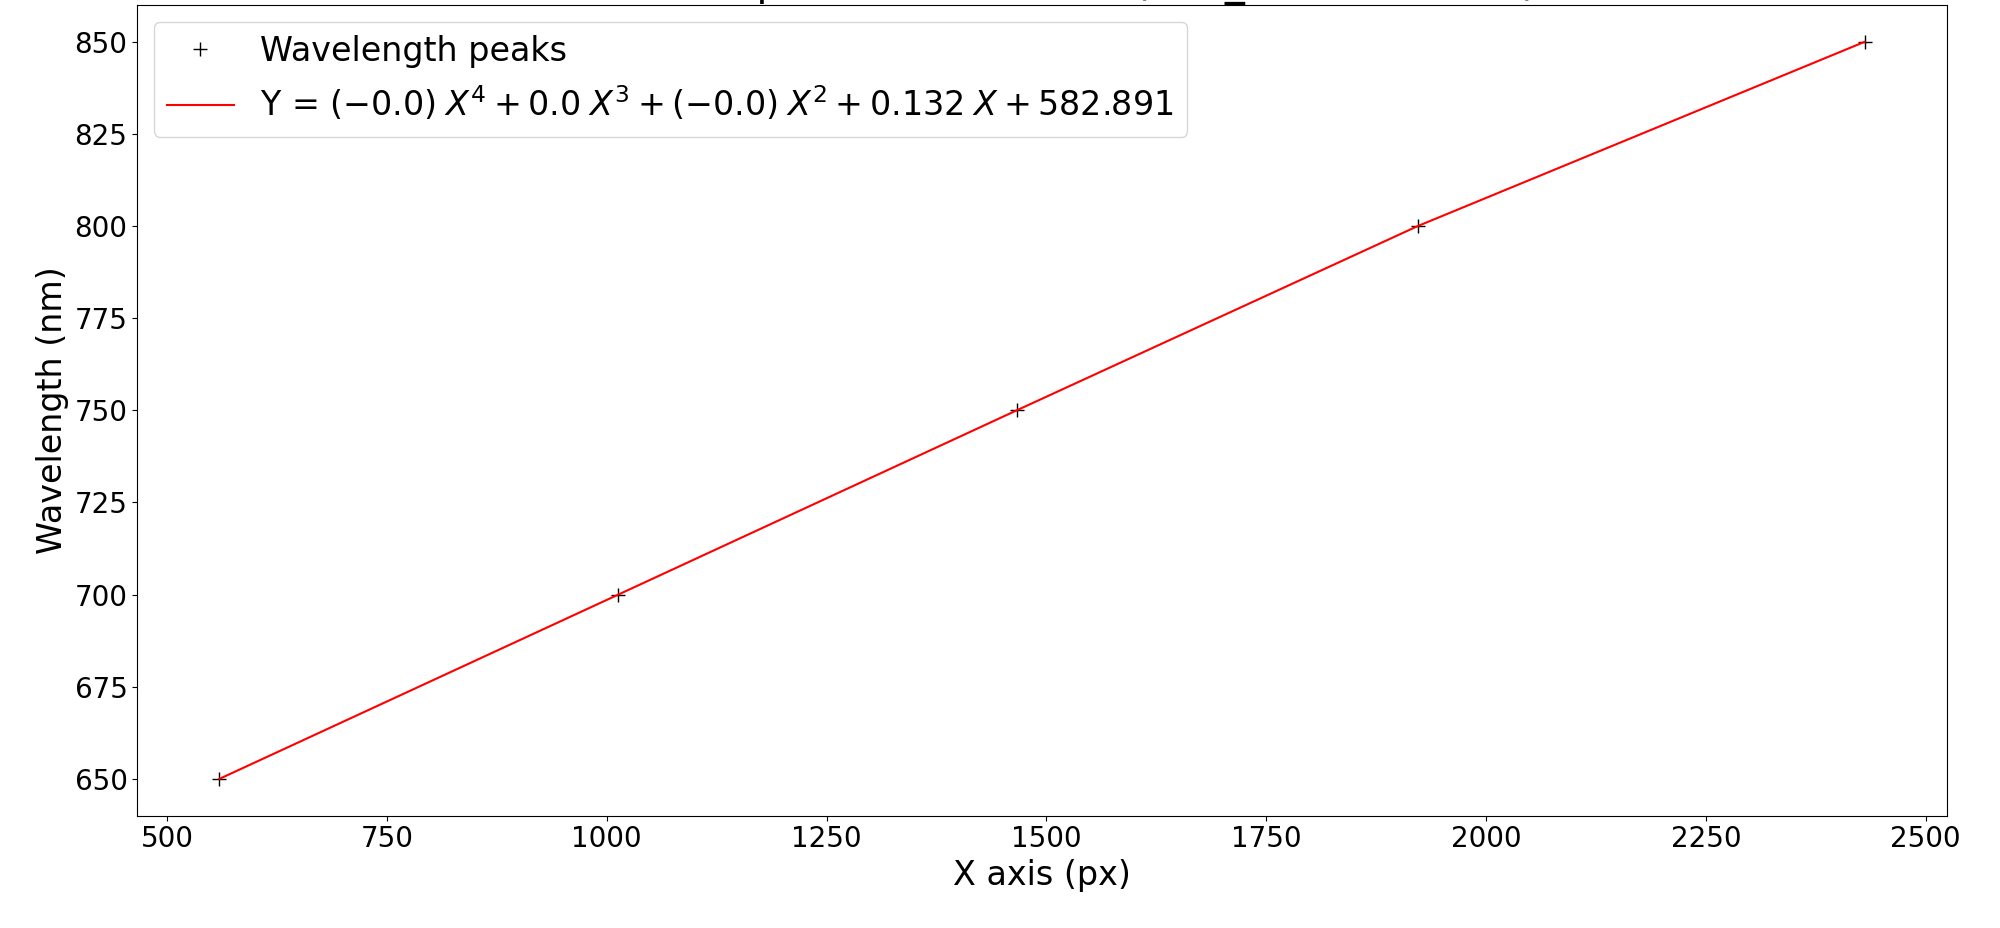
\includegraphics[width=\textwidth]{Figure_Chap5/20220404_5TC_PY_SpectralCalFitFort01_Crop.png}
    \end{subfigure}
    \caption[Étalonnage spectral de FIRSTv2 sur le banc de recombinaison de SCExAO.]{Étalonnage spectral de FIRSTv2 sur le banc de recombinaison de SCExAO. En haut : identification des pics de la source d'étalonnage de l'instrument CHARIS sur les pixels de la caméra pour l'une des sorties de la puce. En bas : les longueurs d’onde en fonction des positions des pics sur la caméra ainsi que l’ajustement polynomial associé.}
    \label{fig:V2SpecCalSubaru}
\end{figure}

Enfin, la figure~\ref{fig:FIRSTV1V2FinalPhoto} présente une photographie du banc de recombinaison de \ac{SCExAO} décrit précédemment par le schéma de principe de la figure~\ref{fig:FIRSTV1V2FinalScheme}. Je ne reviendrai pas sur sa description qui est similaire au premier paragraphe de cette section.

% Photo du banc de recombinaison après intégration du nouveau spectro et de la nouvelle caméra de V2
% + ré-intégration de V1 (>=20220427)
\begin{figure}[ht!]
    \centering
    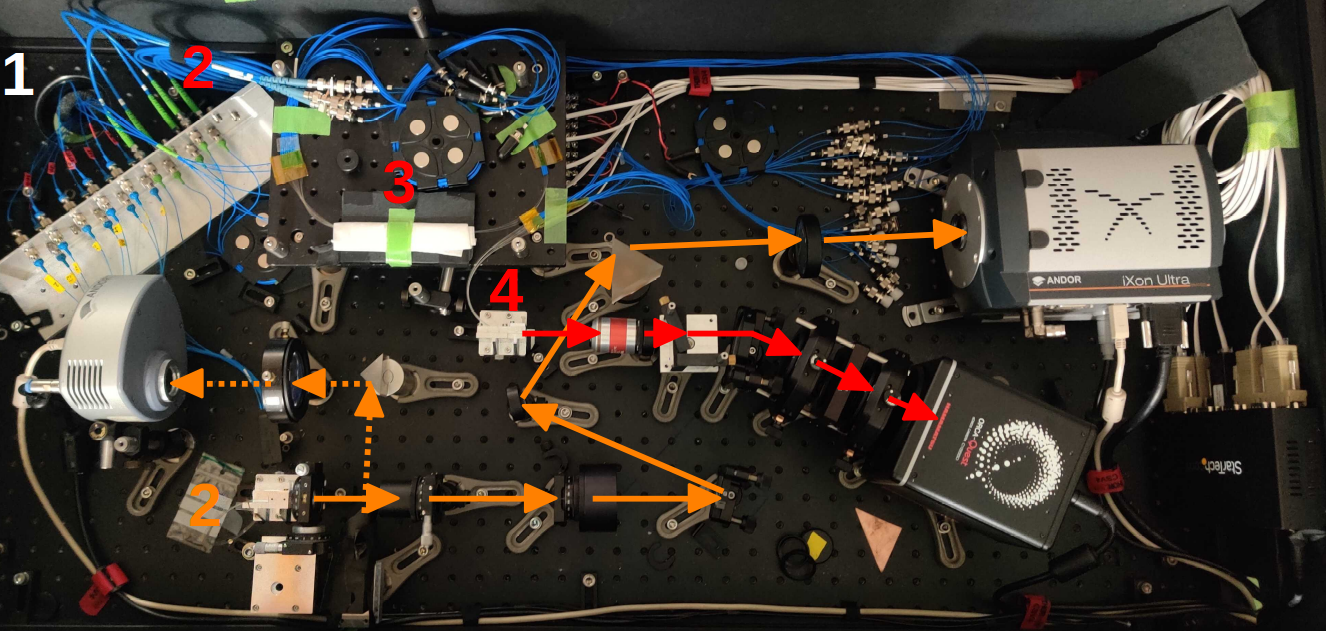
\includegraphics[width=\figwidth]{Figure_Chap5/20220601_SCExAO_FIRSTRecombBench_V1_V2_Photo_label.png}
    \caption[Photographie des deux versions de FIRST installées en parallèle sur le banc de recombinaison de SCExAO.]{Photographie des deux versions de FIRST installées en parallèle sur le banc de recombinaison de SCExAO. Les éléments et chemin optique de FIRSTv1 et FIRSTv2 sont représentés, respectivement, en orange et en rouge. Les fibres (1) proviennent du banc visible. 9 sont connectées au V-Groove de v1 (2) puis un miroir plan mobile permet de diriger les faisceaux vers la voie photométrique (flèches en pointillés) ou vers la voie interférométrique (flèches continues) composée par le système anamorphique, deux miroirs plans, un prisme dispersant, une lentille d'imagerie et une caméra (Andor Ixon). 5 des fibres d'entrée de v2 sont connectées à l'enchaînement de composants : ODLs (2), puce photonique (3) et V-Groove (4). La voie interférométrique de v2 (en rouge) est ensuite composée de l'objectif de microscope, du prisme de Wollaston, du réseau holographique, de deux lentilles d'imagerie et de la caméra (Hamamatsu). Crédit : Sébastien Vievard.}
    \label{fig:FIRSTV1V2FinalPhoto}
\end{figure}


%%%%%%%%%%%%%%%%
\subsection{La configuration des bases}

La configuration des sous-pupilles dont les faisceaux sont recombinés est présentée sur la figure~\ref{fig:SegUVSubaruA}. À la différence de celle qui est choisie sur le banc de test en laboratoire, ici l'ombre de l'obstruction centrale du télescope doit être prise en compte. Celle-ci est visible sur l'image du plan pupille en entrée de la partie de l'injection de \ac{FIRST} (du banc visible de \ac{SCExAO}) montrée en arrière plan. Ainsi, tous les segments de couleur noire ne sont jamais utilisés. Les segments de couleur beige et ceux de couleur verte sont ceux choisis pour la recombinaison de \ac{FIRSTv1} et \ac{FIRSTv2} (numérotés 22, 26, 27, 31 et 35), respectivement. Enfin, le segment rouge est défectueux et les segments bleus ne sont utilisés par aucun des instruments. Ici, la configuration optique est telle que devant chaque segment est alignée une fibre optique du toron. La figure~\ref{fig:SegUVSubaruB} présente le plan UV des fréquences spatiales échantillonnées par les sous-pupilles de \ac{FIRSTv2} précédemment choisies. Les couleurs correspondent aux longueurs d'onde sur la gamme spectrale $600 - 800 \,$nm. Enfin, seules les bases $22 - 26$ et $22 - 35$ sont redondantes, respectivement, avec les bases $35 - 31$ et $26 - 31$.

\begin{figure}[ht!]
    \centering
    \begin{subfigure}[t]{0.43\textwidth}
        \centering
        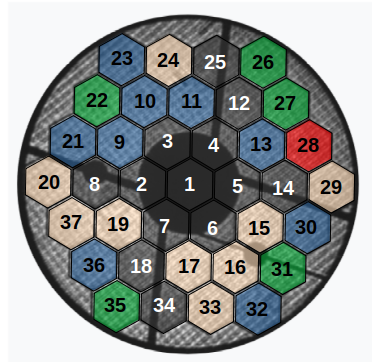
\includegraphics[width=\textwidth]{Figure_Chap5/BaselineMap_Subaru_V1_V2_20221010.png}
        \caption{Configuration des sous-pupilles choisies pour FIRSTv1 (en beige) et FIRSTv2 (en vert) dans le plan pupille du MEMS de FIRST au Subaru. Les segments jamais utilisés sont en noirs (à cause de l'obstruction centrale du télescope, montrée en arrière plan), dysfonctionnel en rouge et disponibles en bleus. Crédit : Sébastien Vievard.}
        \label{fig:SegUVSubaruA}
    \end{subfigure}\hfill
    \begin{subfigure}[t]{0.55\textwidth}
        \centering
        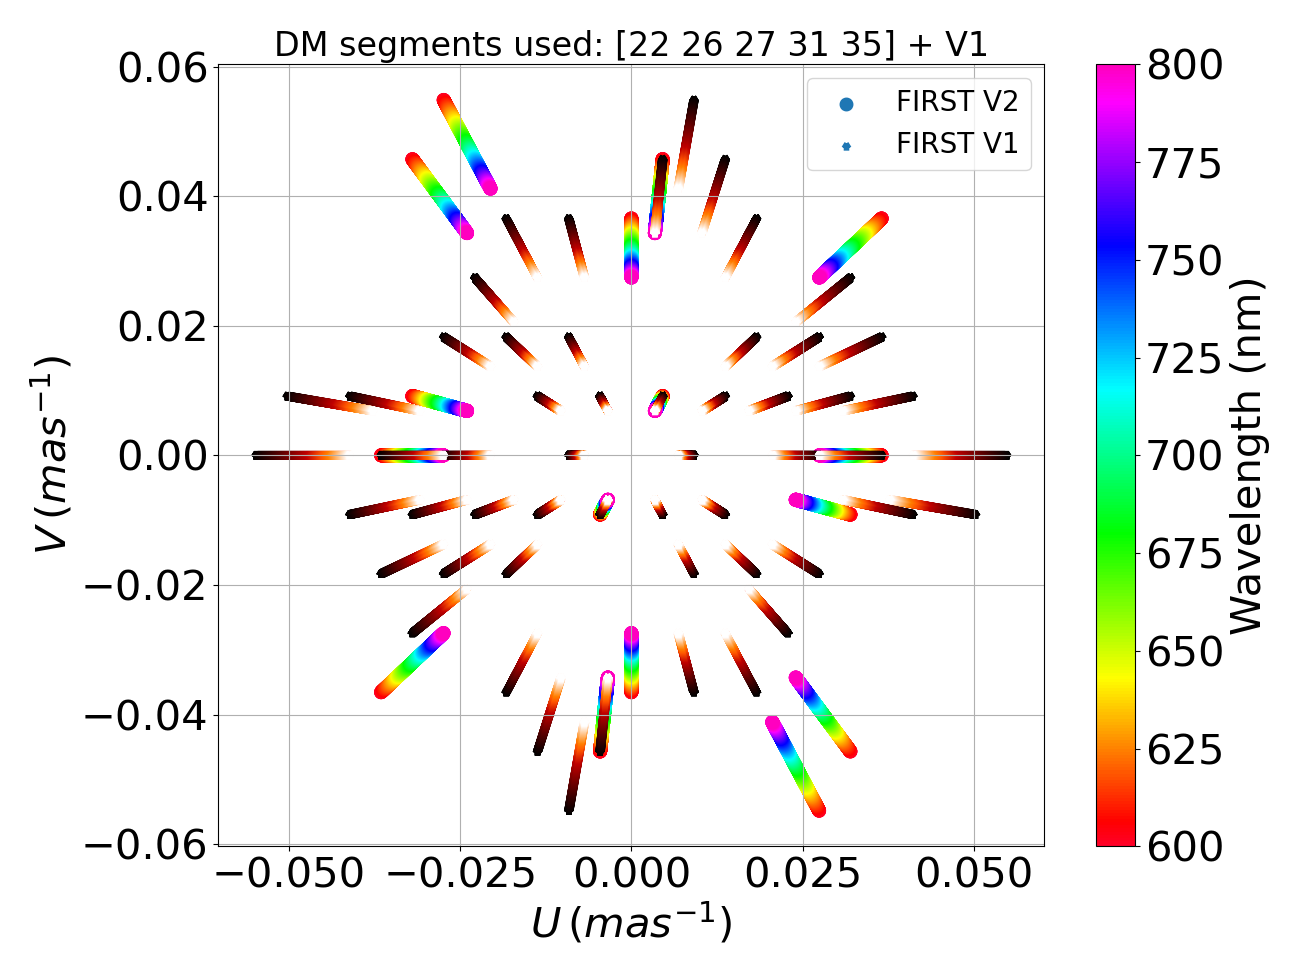
\includegraphics[width=\textwidth]{Figure_Chap5/UVplane_Subaru_22_26_27_31_35_V1.png}
        \caption{Les répartitions des bases choisies pour FIRSTv1 (étoile) et FIRSTv2 (point) représentées dans l'espace de Fourier, appelée aussi la couverture du plan UV des fréquences spatiales. Les couleurs représentent la longueur d'onde (les bandes spectrales sont identiques pour les deux versions).}
        \label{fig:SegUVSubaruB}
    \end{subfigure}
    \caption[Configuration des sous-pupilles et couverture du plan UV de FIRSTv1 et de FIRSTv2 sur SCExAO.]{Configuration des sous-pupilles et couverture du plan UV de FIRSTv1 et de FIRSTv2 sur SCExAO.}
    \label{fig:SegUVSubaru}
\end{figure}


%%%%%%%%%%%%%%%%%%%%%%%%%%%%%%%
\section{Caractérisation de FIRSTv2 sur SCExAO}

%%%%%%%%%%%%%%%%
\subsection{Étude de sensibilité}
\label{sec:V1V2Throughput}

% Mesures pendant la premiere integration à R = 300
On a profité du fait que les deux versions de \ac{FIRST} soient imagées simultanément sur la même caméra (Andor Ixon), comme montré sur la photographie de la figure~\ref{fig:FIRSTV1V2IxonPhoto} de la section~\ref{sec:V1V2Integration}, pour comparer leur sensibilité. La figure~\ref{fig:V1V2Vega} présente une image en échelle logarithmique acquise à un temps d'exposition de $50 \,$ms lors de la nuit d'observation du 24 février 2022 sur l'étoile Véga. La longueur d'onde est selon l'axe horizontal et l'\ac{OPD} selon l'axe vertical pour \ac{FIRSTv1}. Les interférogrammes de \ac{FIRSTv1} et de \ac{FIRSTv2} sont sur la moitié gauche et la moitié droite de l'image, respectivement. Trois sources lasers (de longueurs d'onde $785 \,$nm, $850 \,$nm et $852 \,$nm) sont injectées dans un coupleur fibré intégré juste avant le séparateur \textit{VAMPIRES/FIRST splitter} sur le banc visible (discussion dans la section~\ref{sec:V2SubaruProspectives}), dans le cadre de tests pour la mesure des perturbations de phase induites par des éléments du montage optique, tels que les fibres optiques. Les flux de celles-ci apparaissent comme des colonnes verticales sur la droite des interférogrammes de \ac{FIRSTv1} et comme des points sur la droite des interférogrammes de \ac{FIRSTv2} (indiquées à chaque fois par les flèches rouges).

\begin{figure}[ht!]
    \centering
    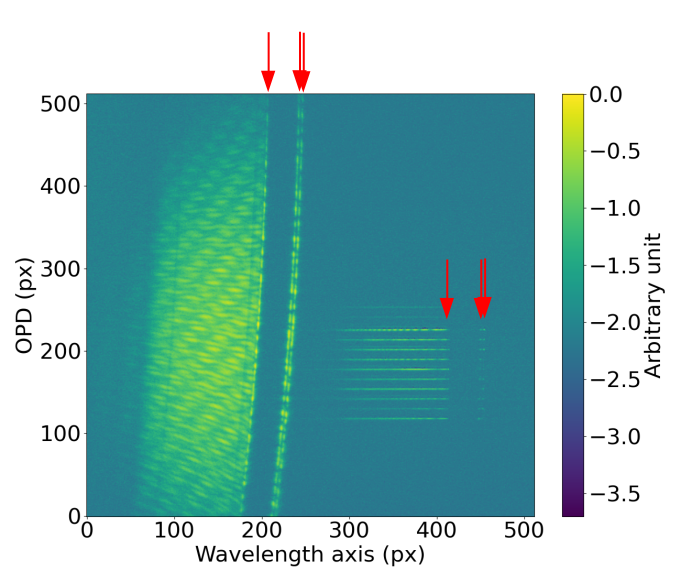
\includegraphics[width=0.8\textwidth]{Figure_Chap5/20220224_Vega_V1V2_FullOn_010_Image100_logscale_arrow.png}
    \caption[Image des interférogrammes des deux versions de FIRST sur la caméra Andor Ixon obtenues lors d'une observation de l'étoile Véga sur SCExAO.]{Image des interférogrammes des deux versions de FIRST sur la caméra Andor Ixon obtenues lors d'une observation de l'étoile Véga sur SCExAO. L'image est normalisée par le flux maximum et est en échelle logarithmique. Les longueurs d'onde et les OPDs (pour FIRSTv1) sont selon les axes horizontal et vertical, respectivement. Les interférogrammes de V1 et de V2 sont imagés sur la moitié gauche et sur la moitié droite de l'image, respectivement. Les flèches rouges montrent les positions des trois sources lasers injectées en entrée de FIRST.}
    \label{fig:V1V2Vega}
\end{figure}

% Estimation du rapport de transmission entre V1 et V2
À partir de cette image, le flux total des deux versions de \ac{FIRST} est calculé en sommant les pixels sur lesquels les interférogrammes sont imagés, en omettant le flux provenant des sources lasers. Ces flux sont ensuite normalisés par le nombre de faisceaux injectés : 9 pour \ac{FIRSTv1} et 5 pour \ac{FIRSTv2}. Enfin, le rapport de ces deux flux normalisés donne une estimation de la différence de transmission entre les deux versions. On estime ainsi que \ac{FIRSTv2} transmet $\sim 20$ fois moins que \ac{FIRSTv1}. De plus, dans cette configuration, les deux versions comprennent les mêmes composants exceptées les \ac{ODL}s et la puce photonique intégrées à \ac{FIRSTv2}. D'après les transmissions des \ac{ODL}s et de la puce $Y$ estimées, respectivement, à $30\%$ (section~\ref{sec:V1V2Integration}) et $15 \%$ (section~\ref{sec:IOChipThroughput}), on s'attend à une transmission de $4,5\%$ par rapport à \ac{FIRSTv1}, ce qui est cohérent avec l'estimation précédente.

Ainsi, avec le nouveau spectro-imageur intégré par la suite, de résolution spectrale égale à $\sim 3\,000$, on s'attend à ce que le flux par pixel soit divisé par 10. Cela a empêché par la suite l'acquisition de données sur ciel après l'intégration du nouveau spectro-imageur montrant bien la nécessité de se passer des \ac{ODL}s et du développement de puce d'optique intégrée plus transmissives.


%%%%%%%%%%%%%%%%
\subsection{Étude de stabilité}
\label{sec:V2StabilitySubaru}

% Perturbations visibles sur les données de fullon
La figure~\ref{fig:FullOnDataSCExAO} présente les données interférométriques acquises sur \ac{FIRSTv2}, sur la source interne de \ac{SCExAO} (la source \sk). La puce $Y$ est installée ainsi que le premier spectro-imageur de résolution spectrale égale à $300$. Chaque graphique de gauche à droite correspond à une base et les graphiques du haut et du bas représentent les interférogrammes mesurés et ajustés, respectivement, selon le processus présenté dans la section~\ref{sec:FullOnFit}. L'acquisition de ces données est effectuée avec la séquence de modulation à $20$ pas (axe horizontal sur les images de la figure~\ref{fig:FullOnDataSCExAO}), représentée par la figure~\ref{fig:ModSeq20}, avec un temps d'exposition de la caméra égal à $20 \,$ms à une fréquence de $16,45 \,$Hz. Ainsi, entre chaque point de mesure s'écoule $60 \,$ms et un interférogramme est acquis en $1,2 \,$s (correspondant à $20$ points de mesure).

\begin{figure}[ht!]
    \centering
    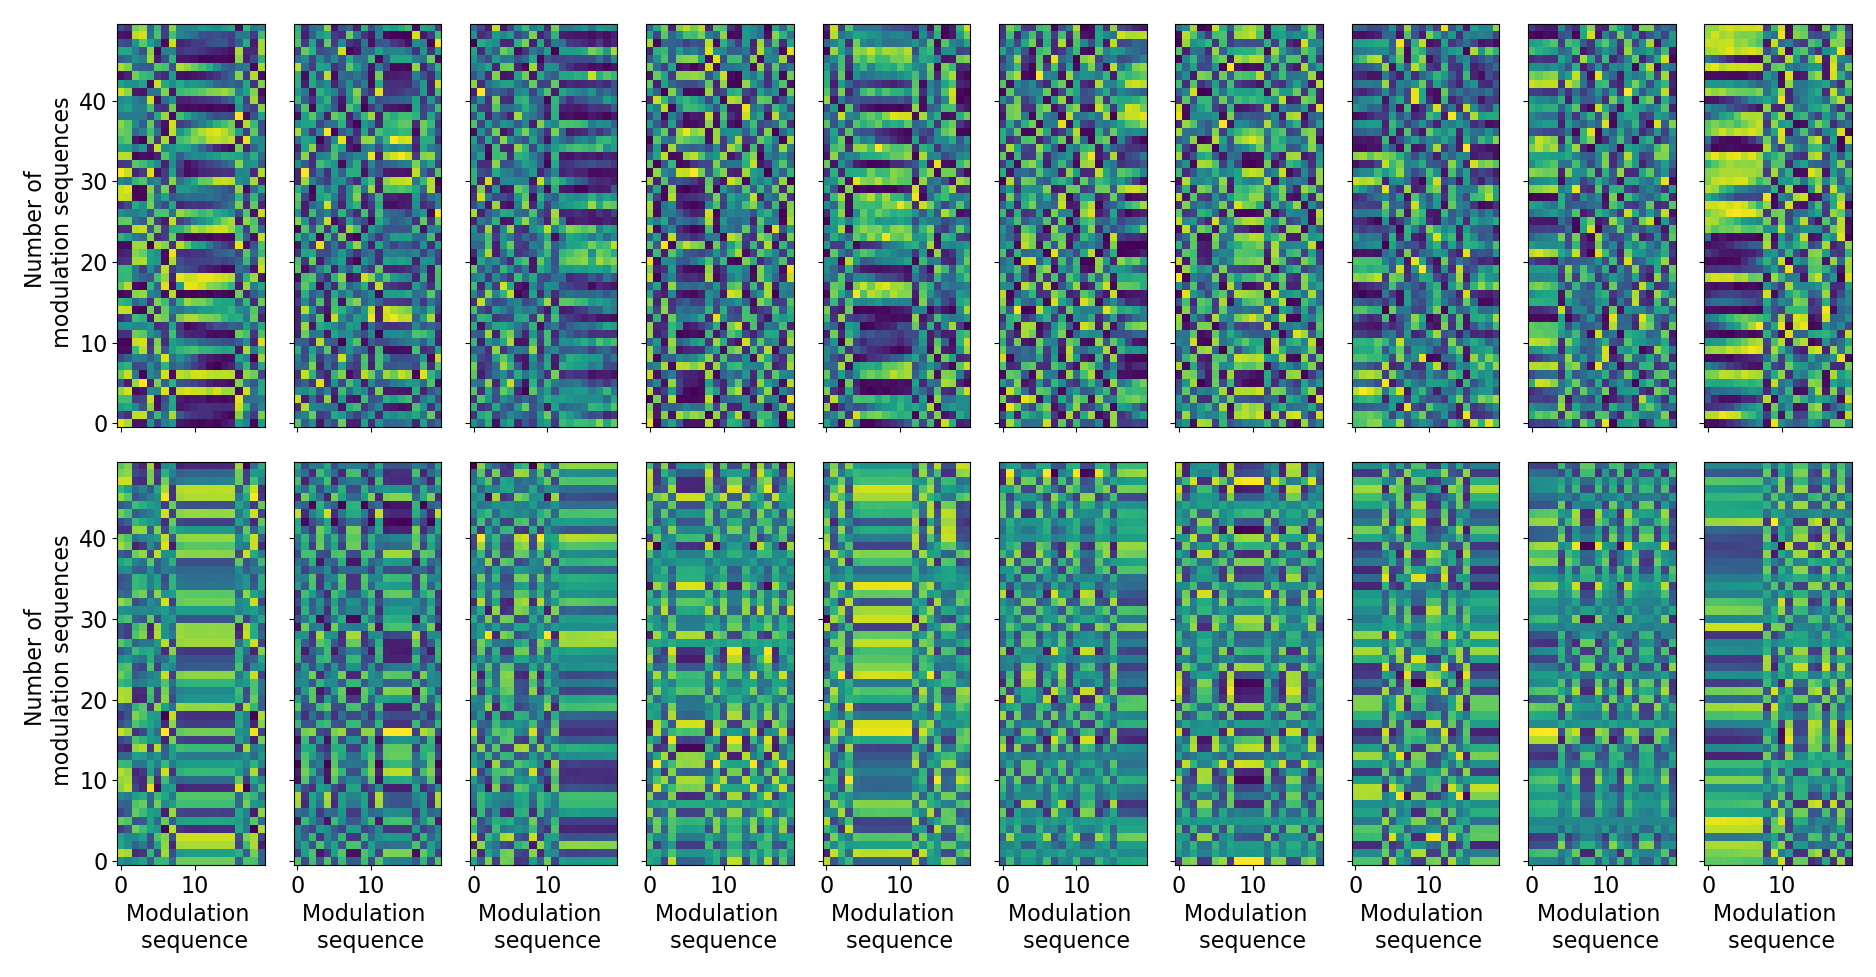
\includegraphics[width=\figwidth]{Figure_Chap5/20220225_SuperK_FringeFitting_TemporalModulation_Pola1_Base_LaTex.png}
    \caption[Images des interférogrammes mesurés et ajustés, avec la puce $Y$ sur la source interne de SCExAO.]{Images des interférogrammes mesurés (lignes du haut) et ajustés (lignes du bas) sur les $10$ bases (en colonne), avec la puce $Y$ et la source interne de SCExAO. Les axes horizontal et vertical représentent, respectivement, la séquence de modulation et le nombre de fois que la séquence de modulation a été acquise. Ces images sont pour le canal spectral $\sim 700 \,$nm.}
    \label{fig:FullOnDataSCExAO}
\end{figure}

La figure~\ref{fig:FullOnData} présente les mesures effectuées en laboratoire, équivalentes à celles montrées ici, sur la puce $Y$ (figure du haut), avec le spectro-imageur de résolution spectrale égale à $\sim 3\,200$, pour un temps d'exposition de la caméra de $100 \,$ms à une fréquence de $9,9 \,$Hz. Chaque point est donc acquis toutes les $101 \,$ms et un interférogramme toutes les $1,2 \,$s, ce qui est similaire aux données présentées sur la figure~\ref{fig:FullOnDataSCExAO}. Par comparaison visuelle des images des interférogrammes de ces deux prises de données, on remarque que ceux estimés sur \ac{FIRSTv2} intégré sur \ac{SCExAO} présentent une plus grande perturbation en fonction du temps (axe vertical). 

% Mesure de CP
On s'en rend bien compte en traçant l'\ac{OPD} estimé à partir de l'ajustement des phases des interférogrammes, en fonction du temps. En suivant la même procédure que dans la section~\ref{sec:CPStabilityMeudon}, sur les données montrées dans le paragraphe précédent, on obtient les graphiques de l'évolution de l'\ac{OPD} et des clôtures de phase en fonction du temps, présentés sur la figure~\ref{fig:OPDfitVStimeSubaru}. Cette dernière est similaire à la figure~\ref{fig:OPDfitVStime}, pour les dix bases. Les courbes d'\ac{OPD} présentent des pics qui restent présents dans les courbes de clôtures de phase. Ces pics apparaissent lorsque l'estimation de la phase échoue. En retirant ces points extrêmes on estime l'écart-type de la clôture de phase en moyenne égal à $\sim 1,3 \,$\um~rms, contre $\sim 50 \,$nm rms estimé en laboratoire.

\begin{figure}[ht!]
    \centering
    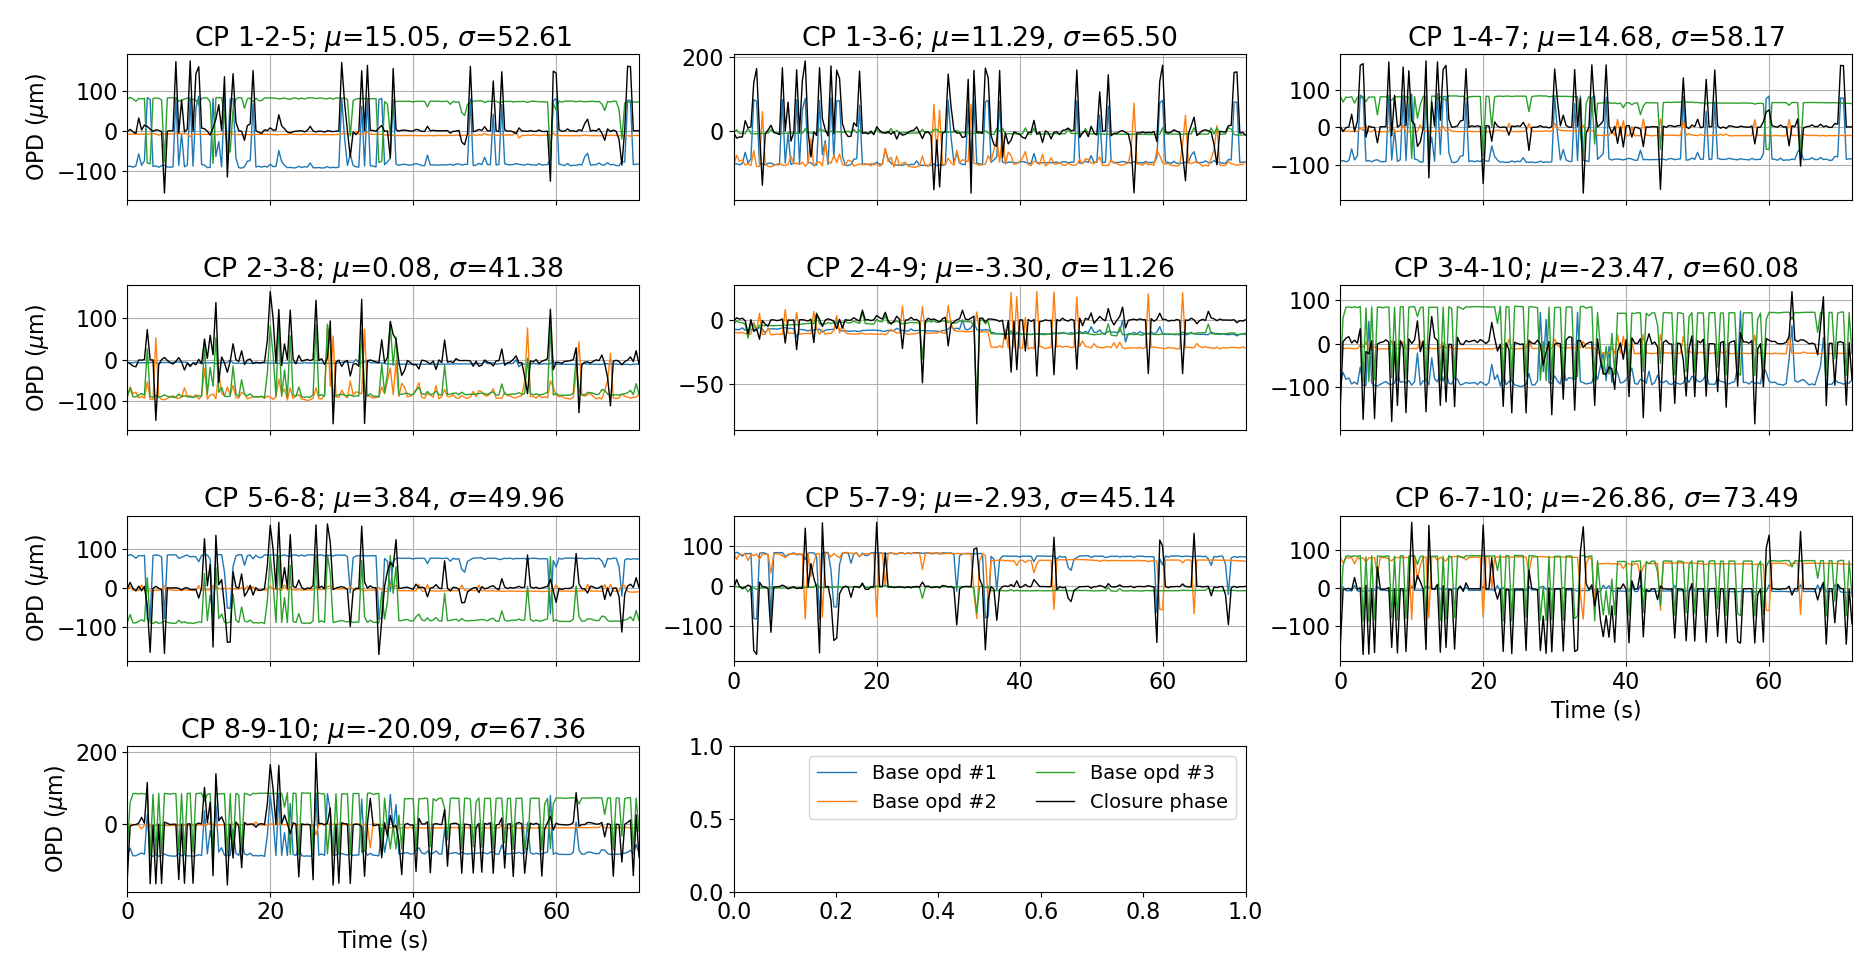
\includegraphics[width=\figwidth]{Figure_Chap5/20220225_SuperK_FullOnData_OPDFitCPvsTime_Pola1_Base_LaTex.png}
    \caption[Graphiques de l'OPD en fonction du temps des dix triangles formés par les dix bases de FIRSTv2 sur la source interne de SCExAO avec la puce $Y$, avant la protection des fibres.]{Graphiques de l'OPD en fonction du temps (tracé en couleur) des dix triangles formés par les dix bases de FIRSTv2 sur la source interne de SCExAO avec la puce $Y$, avant la protection des fibres contre les caméras de VAMPIRES. Les clôtures de phase sont tracées en noir et leur valeur moyenne et l'écart-type sont écrits dans les sous-titres. Les courbes sont tracées pour $4\,000$ images de temps d'exposition égal à $20 \,$ms.}
    \label{fig:OPDfitVStimeSubaru}
\end{figure}

% Origines et solutions
Il est très probable que ce soit les fibres qui sont sensibles aux perturbations qui induisent ces pics observés dans les mesures d'\ac{OPD} en ajoutant un bruit trop important sur les phases estimées. Avant que \ac{FIRSTv2} soit intégré sur \ac{SCExAO}, les fibres optiques qui se trouvent dans la transition entre le banc visible et le banc de recombinaison de \ac{FIRST} (se trouvant donc à l'extérieur des coffrages) avaient déjà été protégées en les plaçant dans un tube en mousse, afin de les protéger des courants d'air se trouvant sur la plateforme Nasmyth du télescope. On pense donc que ce sont les ventilateurs des caméras de l'instrument \ac{VAMPIRES} sur le banc visible qui seraient (au moins en partie) à l'origine de ces perturbations car les fibres du toron en sont à proximité. Celles-ci ont donc aussi été protégées sur le banc visible et de nouvelles mesures, présentées sur la figure~\ref{fig:OPDfitVStimeSubaruProtect}, montrent des courbes présentant moins de pics extrêmes. Malgré cela, la stabilité n'est pas améliorée car l'écart-type moyen des clôtures de phase (après avoir retiré les pics) est estimé à $\sim 2 \,$\um~rms. De plus, l'écart-type des clôtures de phase a été estimé à $\sim 66 \,$nm sur \ac{FIRSTv1}. Ainsi, ces perturbations ont probablement lieu au niveau des \ac{ODL}s ou la méthode d'acquisition des interférogrammes par la modulation des franges en est peut-être trop sensible. D'autres tests sont ainsi nécessaires pour identifier la source de ces perturbations et améliorer la stabilité des mesures sur \ac{FIRSTv2}.

\begin{figure}[ht!]
    \centering
    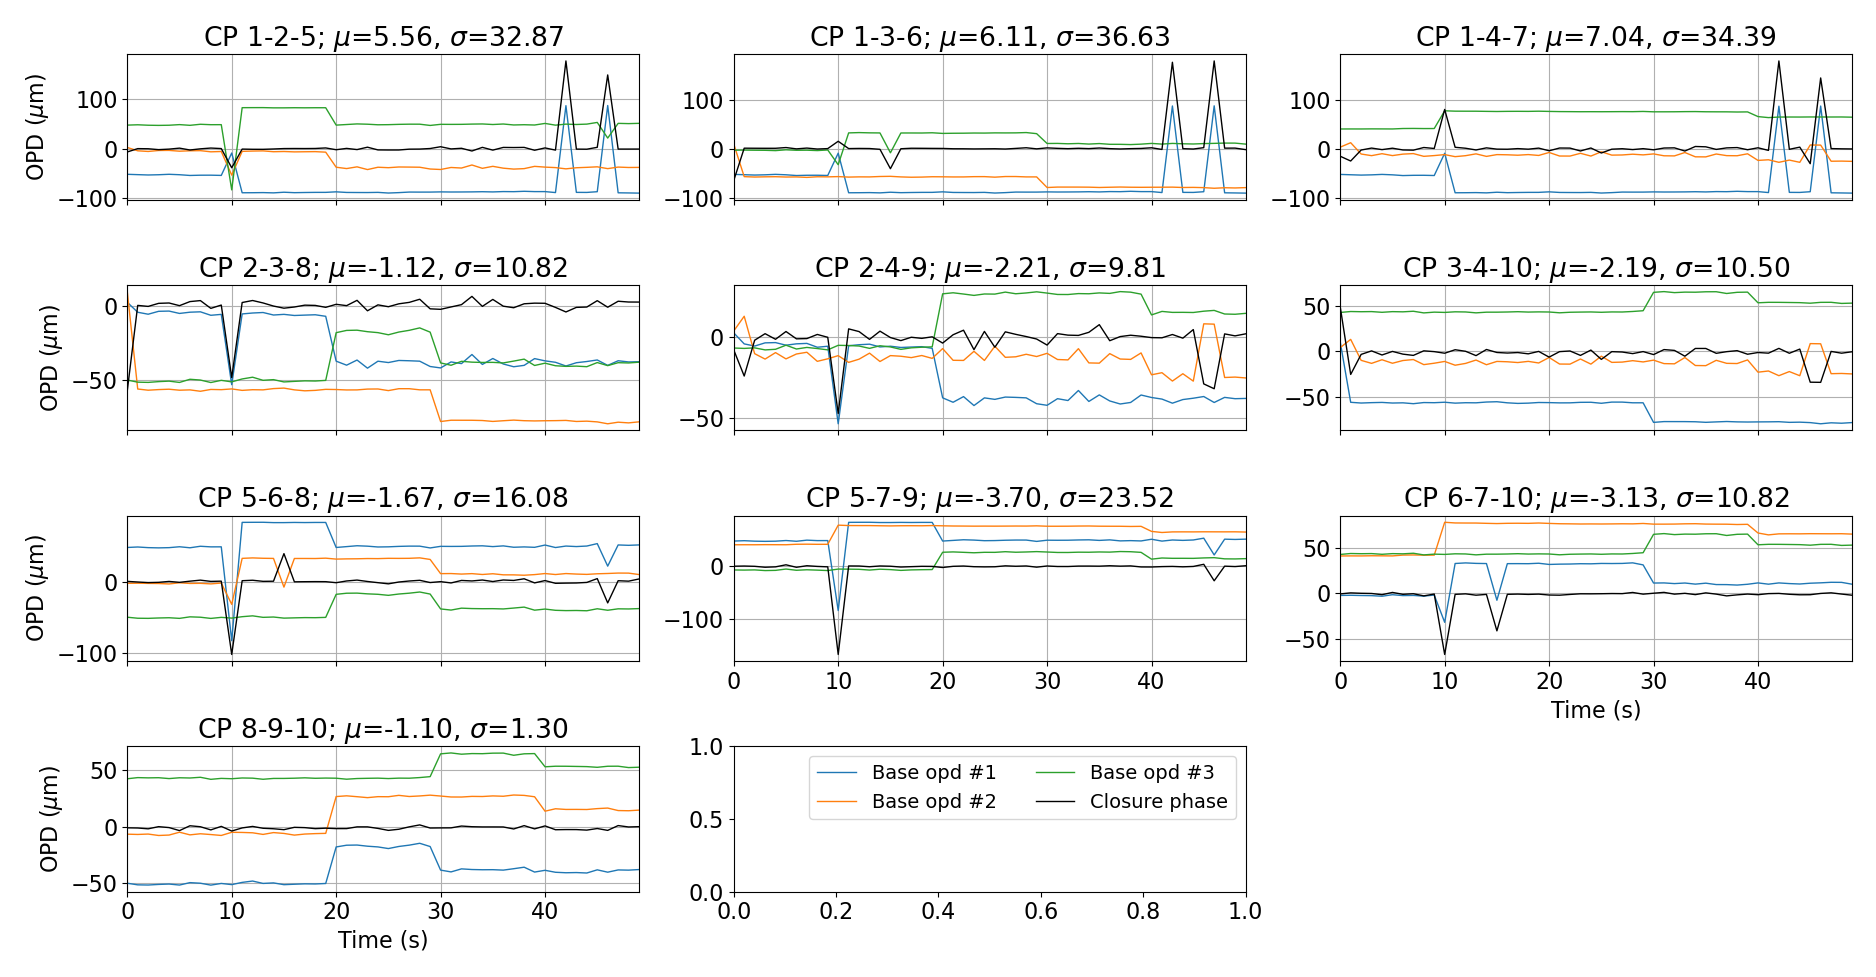
\includegraphics[width=\figwidth]{Figure_Chap5/20220404_FullOnData_OPDFitCPvsTime_Pola1_Base_LaTex.png}
    \caption[Graphiques de l'OPD en fonction du temps des dix triangles formés par les dix bases de FIRSTv2 sur la source interne de SCExAO avec la puce $Y$, après la protection des fibres.]{Graphiques de l'OPD en fonction du temps (tracé en couleur) des dix triangles formés par les dix bases de FIRSTv2 sur la source interne de SCExAO avec la puce $Y$, après la protection des fibres contre les caméras de VAMPIRES. Les clôtures de phase sont tracées en noir et leur valeur moyenne et l'écart-type sont écrits dans les sous-titres. Les courbes sont tracées pour $1\,000$ images de temps d'exposition égal à $50 \,$ms.}
    \label{fig:OPDfitVStimeSubaruProtect}
\end{figure}


%%%%%%%%%%%%%%%%%%%%%%%%%%%%%%%
\section{Première lumière au télescope Subaru}

% Première lumière le 10 septembre 2021 (AlphaPer)
La première lumière de \ac{FIRSTv2} a eu lieu le 10 septembre 2021, par l'observation de $\upalpha$ Per. La figure~\ref{fig:V2FirstLight} présente une image de cette première lumière, à un temps d'exposition égal à $100 \,$ms et un gain \textit{EM} de la caméra de $300$. Seuls les faisceaux des sous-pupilles de la première base (formée par les segments 26 et 27) sont injectés dans les fibres induisant la formation des franges sur la base en bas de l'image. Sur la partie gauche de l'image apparaît la lumière des trois lasers de longueurs d'onde $785 \,$nm, $850 \,$nm et $852 \,$nm, injectés sur l'instrument pour effectuer des tests sur la mesure de la perturbation de la phase sur le banc (voir plus de détails dans la section~\ref{sec:V2SubaruProspectives}).

\begin{figure}[ht!]
    \centering
    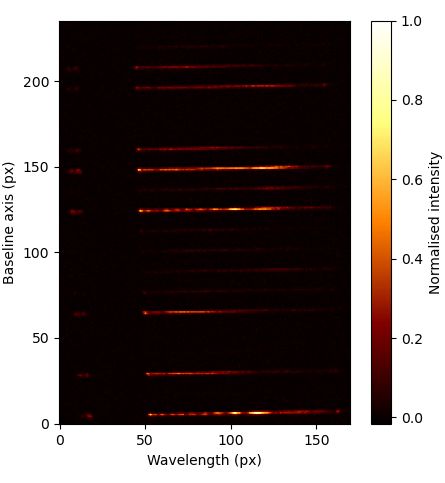
\includegraphics[width=\figwidth]{Figure_Chap5/20210910_AlphaPer_ODLseq1_Base1_2_Image001.png}
    \caption[Image des sorties de la puce $X$ lors de la première lumière de FIRSTv2 sur SCExAO sur l'étoile Alpha Per, le 21 septembre 2021.]{Image des sorties de la puce $X$ lors de la première lumière de FIRSTv2 sur SCExAO sur l'étoile Alpha Per, le 21 septembre 2021. Seuls les faisceaux des sous-pupilles 26 et 27 formant la première base sont injectés. La base est imagée en bas de l'image et des franges d'interférence sont visibles. Le temps d'exposition est de $100 \,$ms et le gain \textit{EM} de la caméra vaut 300.}
    \label{fig:V2FirstLight}
\end{figure}

Par la suite, nous avons observé avec \ac{FIRSTv2} des étoiles brillantes telles que Véga et Capella. Les données acquises n'ont pas permis d'estimer des courbes de phase mais nous ont permis d'améliorer l'exploitation de l'instrument d'un point de vue instrumental et d'un point de vue logiciel. 

% Nécessité de protéger les fibres optiques
En effet, ce qui a été identifié comme le plus critique est sans doute l'isolation des fibres optiques des perturbations de leur environnement. Comme discuté dans la section~\ref{sec:V2StabilitySubaru}, elles sont sensibles aux mouvements d'air générés par les différentes caméras (trois sont, par exemple, installées sur le banc de recombinaison) et les vibrations probablement transmises sur le banc de recombinaison vissé sur \ac{SCExAO} ainsi qu'aux autres instruments (voir la photographie de la figure~\ref{fig:SCExAOPhoto}). Une nette amélioration a déjà été observée (figure~\ref{fig:OPDfitVStimeSubaruProtect}) après la protection des fibres de \ac{FIRST} sur le banc visible mais il reste encore à protéger les fibres présentes sur le banc de recombinaison, qui sont plus longues dans le cas de \ac{FIRSTv2}, à cause des \ac{ODL}s. Mais encore, la méthode de reconstruction des interférogrammes par modulation des franges est probablement sensible aux résidus de phase en aval du système d'optique adaptative, empêchant l'estimation des courbes de phase lors du traitement de données. D'autres solutions à ce sujet pourraient être envisagées comme l'utilisation d'une puce photonique dite \textit{ABCD} (voir la section~\ref{sec:V2SubaruProspectives}).

% Nécessité du polariseur + Wollaston (<20220214)
De plus, il est primordial de disposer d'un prisme de Wollaston en sortie du V-Groove connecté à la puce afin de séparer les deux polarisations sur la caméra et de les traiter séparément. Un tel prisme n'a pu être installé qu'en mars 2022 et toutes les données qui précèdent cette date ne sont pas exploitables.

% Nécessité de connaître le step de modulation sur chaque image acquise (<20220225)
Enfin, lors du traitement des données, l'étape de modulation des franges doit être identifiée à chaque image. La matrice des données doit contenir les franges modulées de la même façon que les franges d'étalonnage contenues dans la \ac{P2VM} lors de l'ajustement des franges décrit dans la section~\ref{sec:FullOnFit}. Durant quelques nuits d'observation, la construction du logiciel ne permettait pas de connaître les étapes de la séquence de modulation de chaque image acquises et les données ne peuvent donc pas être traitées.


%%%%%%%%%%%%%%%%%%%%%%%%%%%%%%%%
\section{Perspectives}
\label{sec:V2SubaruProspectives}

Mon projet de thèse a permis d'effectuer certains progrès sur l'implémentation de \ac{FIRSTv2} sur ciel, que j'ai exposé dans ce chapitre. J'expose ici les futurs développement prévus.

% Nessécité d'améliorer les performances en transmission (retirer les odls, utiliser de nouvelles puces transmissives)
L'aspect le plus urgent est l'augmentation de la transmission de \ac{FIRSTv2}. Comme nous l'avons vu, la configuration actuelle de l'instrument ne permet pas d'obtenir un signal avec un \ac{SNR} suffisant. Nous prévoyons ainsi de retirer les lignes à retard de l'instrument car elles sont trop peu transmissives ($\sim 30\%$). Les solutions possibles ont été discutées dans la section~\ref{sec:ODLDiscussions}. De plus, l'équipe travaille à de nouvelles puces photoniques plus transmissives comme je l'ai exposé dans la section~\ref{sec:ChipCharacDiscu}.

% Métrologie pour la mesure des perturbations de phase sur le banc afin de les compenser au traitement
Quatre sources lasers pour des mesures de métrologie sont installées afin de tirer profit des mesures d'\ac{OPD} entre les paires de sous-pupilles permises par \ac{FIRST} pour mesurer les perturbations du front d'onde incident et tenter de les corriger. De cette manière, \ac{FIRST} pourrait fournir simultanément des données scientifiques et des informations sur le front d'onde incident qui seraient utilisées par un système de correction d'optique adaptative \citep{vievard2021}. Les longueurs d'onde des quatre sources lasers sont $642 \,$nm, $785 \,$nm, $850 \,$nm et $852 \,$nm. Les deux sources émettant dans les deux dernières longueurs d'onde sont couplées dans la même fibre grâce à un coupleur $Y$ dont la sortie est combinée avec les deux autres sources grâce à un composant de multiplexage en longueur d'onde (\ac{WDM}). Les quatre sources lasers sont ainsi combinées dans une unique fibre optique qui est intégrée sur le banc visible de \ac{SCExAO} directement en amont du séparateur de faisceau entre les instruments \ac{FIRST} et \ac{VAMPIRES}, nommé \textit{VAMPIRES/FIRST splitter} sur le schéma de la figure~\ref{fig:SCExAOScheme}. Les quatre sources peuvent ainsi être imagées sur la caméra avec les franges interférences et un programme de traitement de données additionnel pourrait permettre de connaître les perturbations présentes sur le banc que subissent les mesures de phase en temps réel afin de les corriger. De premiers tests à ce sujet ont été faits durant ma thèse mais n'ont pour l'instant pas fonctionné car les courbes de phase estimées sont très repliées à cause de la difficulté d'obtenir l'\ac{OPD} nulle entre tous les faisceaux.

% Développement du nouveau logiciel de contrôle de FIRST pour l'adapter au calcul rapide synchronisé avec CACAO
Comme discuté dans le paragraphe précédent, un des projets en cours concerne l'exploitation de \ac{FIRST} comme un senseur de front d'onde. Pour cela, un ordinateur de contrôle dédié à cela a été acquis pour augmenter la cadence de calculs et la synchronisation avec les autres composants et processus de \ac{SCExAO} (e.g. avec le miroir déformable pour la correction par optique adaptative, le logiciel \ac{CACAO} \citep{guyon2020}). Dans ce but, de nouveaux développements doivent être effectués sur le logiciel de contrôle de \ac{FIRST}. L'augmentation de la puissance de calcul pourrait aussi permettre une augmentation de la fréquence de modulation des franges lors de l'acquisition des images interférométriques, à condition que l'instrument soit plus transmissif. Les interférogrammes mesurés ne seraient donc plus affectés par les résidus des perturbations atmosphériques, pour des fréquences d'acquisition supérieures à quelques centaines d'images par seconde.

% Utilisation de puce ABCD pour éviter la modulation, diminuer la quantité de données nécessaire (d'un facteur 4)
Enfin, les développements s'orientent vers la fabrication de puces photoniques dites \textit{ABCD}. Une telle puce fournit quatre sorties par base déphasées de $\uppi / 2 \,$rad et permet la mesure complète d'une frange sur une unique image. Cette technique est aussi mentionnée dans la section~\ref{sec:ChipCharacDiscu}. Elle permet ainsi de diviser par 12 la quantité de données à acquérir pour 10 bases, tout en permettant de s'affranchir des perturbations sur les mesures de phases qui ont lieu sur la version actuelle de \ac{FIRSTv2} au cours de l'application de la séquence de modulation des franges (nécessitant 12 images).


